% Chapter 3 — Phương pháp và thiết kế hệ thống

\chapter{Phương pháp và thiết kế hệ thống}
\label{Chapter3}

%----------------------------------------------------------------------------------------

\begin{figure}[H]
    \centering
    \includegraphics[width=1\linewidth]{src//images//chapter3/fig1_pipeline.png}
    \caption{Kiến trúc tổng quan hệ thống kiểm thử xâm nhập đa tác nhân}
    \label{fig:fig1_pipeline}
\end{figure}

\textbf{Hình \ref{fig:fig1_pipeline}} thể hiện kiến trúc tổng quan của hệ thống, được tổ chức theo mô hình pipeline tuyến tính gồm năm giai đoạn nối tiếp nhau: (1) thu thập thông tin (Reconnaissance), (2) đặt giả thuyết (Hunt), (3) sắp xếp ưu tiên (Coordinate), (4) vòng lặp khai thác per-bug (Debate → Exec → Verify), và (5) tổng hợp báo cáo (Report). Điểm cốt lõi trong thiết kế là sự phân tách rõ ràng giữa phần LLM đảm nhiệm việc suy luận ngữ cảnh trong từng ô xử lý, và phần code tất định đảm nhiệm toàn bộ việc điều phối luồng và ra quyết định cuối cùng về kết quả khai thác.

Để giải quyết bài toán phức tạp về việc phát hiện và khai thác các lỗ hổng Broken Access Control và Business Logic Flaw trên các ứng dụng web hiện đại, hệ thống được thiết kế theo một khung phương pháp luận toàn diện, mô phỏng lại quá trình tư duy, lập kế hoạch và thử nghiệm khai thác thực tế của một chuyên gia phân tích bảo mật --- thay vì rập khuôn theo các tải trọng cố định như công cụ quét truyền thống. Quy trình vận hành của hệ thống được tổ chức xoay quanh ba trụ cột chính, bắt đầu từ việc trinh sát thu thập bằng chứng, tiếp nối bằng quá trình tranh luận tư duy đa chiều, và chốt lại bằng cơ chế xác minh tự động.

\textit{Trụ cột thứ nhất} giải quyết bài toán thiếu hụt thông tin ngữ cảnh thông qua tác tử trinh sát tự động: hệ thống duyệt toàn bộ cấu trúc trang web mục tiêu dưới nhiều góc độ tài khoản và phiên làm việc khác nhau, tạo ra mạng lưới bằng chứng phong phú về cách hệ thống phân quyền và xử lý nghiệp vụ. \textit{Trụ cột thứ hai} là mô hình luồng tranh luận đa tác tử được quản lý bởi đồ thị trạng thái LangGraph: đội tấn công và đội phòng thủ cọ xát nhau, buộc hệ thống AI phải đào sâu suy nghĩ và loại bỏ các giả thuyết hời hợt. \textit{Trụ cột thứ ba} thiết lập cơ chế xác minh hai tầng: tầng lọc tất định bằng mã nguồn (ProofGate) đối chiếu thay đổi trạng thái HTTP trước, sau đó tầng cố vấn LLM đánh giá tính nghiêm trọng --- hệ thống không tin tưởng tuyệt đối vào bất kỳ quyết định AI nào nếu thiếu bằng chứng thực thi.

%----------------------------------------------------------------------------------------
\section{Tổng quan kiến trúc hệ thống}
%----------------------------------------------------------------------------------------

Hệ thống được xây dựng dựa trên ba nguyên lý thiết kế cốt lõi, mỗi nguyên lý giải quyết một điểm yếu căn bản của các công cụ kiểm thử tự động truyền thống.

\textbf{Nguyên lý thứ nhất: Dữ liệu HTTP thật là sự thật duy nhất.} Các công cụ tự động hóa hiện có thường để AI tự đánh giá liệu một endpoint có bị khai thác thành công hay không, dẫn đến tỷ lệ false positive cao do mô hình ngôn ngữ có xu hướng tự tin ngay cả khi không có bằng chứng rõ ràng. Hệ thống này đảo ngược hoàn toàn cách tiếp cận đó: phán quyết cuối cùng về \textit{``lỗ hổng đã bị khai thác''} được đưa ra bởi một thành phần code tất định gọi là \textit{ProofGate}, thành phần này đọc trực tiếp từng HTTP request/response thực tế và kiểm tra các điều kiện cụ thể như \textit{``response 200 với body chứa email của nhiều người dùng''} hoặc \textit{``số tiền âm được server chấp nhận và ghi nhận thay đổi số dư''}. LLM chỉ đóng vai trò tư vấn bổ sung, không có quyền ghi đè kết quả của gate.

\textbf{Nguyên lý thứ hai: Code điều phối, LLM chỉ suy nghĩ trong từng ô.} Thay vì để một LLM tổng quản lý toàn bộ quy trình, hệ thống sử dụng LangGraph để xây dựng một đồ thị trạng thái (\textit{StateGraph}) tất định. Mỗi node trong đồ thị là một hàm Python xử lý một nhiệm vụ cụ thể; mỗi cạnh là một hàm điều kiện Python thuần túy đọc giá trị enum từ trạng thái hiện tại để quyết định node tiếp theo. Không có LLM nào được phép nói \textit{``bây giờ hãy chuyển sang bước xác minh''} hay \textit{``bug này không cần thực thi''}. Điều này đảm bảo tính tái lập và ngăn chặn hiện tượng LLM tự ý bỏ qua các bước kiểm tra quan trọng.

\textbf{Nguyên lý thứ ba: Không cắt bỏ dữ liệu HTTP.} Mọi response body nhận được trong quá trình khai thác được lưu nguyên vẹn trên đĩa, đánh địa chỉ bằng hash SHA-256 trong một kho lưu trữ nội dung (\textit{BodyStore}). Các object trong bộ nhớ chỉ giữ con trỏ (hash + 200 byte đầu + 200 byte cuối), không bao giờ chứa nội dung đầy đủ. Flag \texttt{truncated} luôn bằng \texttt{False} --- không có ngoại lệ. Nguyên lý này ngăn chặn tình huống ProofGate đọc nhầm do dữ liệu bị cắt nửa chừng, đảm bảo zero false positive từ phía gate.

\subsection{Kiến trúc ba tầng}

Hệ thống được phân chia thành ba tầng trách nhiệm độc lập. \textbf{Tầng 1} là lớp code tất định đảm nhiệm việc thu thập bằng chứng (crawler, recorder) và điều phối luồng (LangGraph router). \textbf{Tầng 2} là lớp LLM với bảy vai trò agent --- Crawler, Hunter (đặt giả thuyết), Red (lập kế hoạch tấn công), Blue (phản biện kế hoạch), Exec (thực thi khai thác bằng tool-calling), Verifier (tư vấn xác minh), và Reporter (tổng hợp báo cáo) --- trong đó năm agent chuyên biệt (Hunter, Red, Blue, Exec, Verifier) đảm nhiệm việc suy luận ngữ cảnh, mỗi agent chỉ có thể quan sát và xử lý dữ liệu trong phạm vi nhiệm vụ của mình. \textbf{Tầng 3} là lớp code tất định thứ hai gồm ProofGate và bộ phân loại thực thể (Classifier), đưa ra phán quyết cuối cùng dựa trên bằng chứng HTTP thô.

\subsection{Máy trạng thái vòng đời khai thác}

Mỗi giả thuyết lỗ hổng (BugDossier) trải qua một vòng đời được quản lý bởi một máy trạng thái hữu hạn, được khai báo dưới dạng một từ điển tĩnh (\texttt{TRANSITIONS}) trong mã nguồn. Máy trạng thái gồm mười một trạng thái có thể đạt được qua bảng chuyển: \textit{Queued} (xếp hàng chờ), \textit{Debating} (đang tranh luận), \textit{DebateApproved} (kế hoạch được duyệt), \textit{Executing} (đang thực thi), \textit{Verifying} (đang xác minh), \textit{Exploited} (khai thác thành công), \textit{InfoExposureOnly} (chỉ lộ thông tin), \textit{NotExploited} (không khai thác được), \textit{ProofQualityFail} (bằng chứng không đạt), \textit{SkippedNoEvidence} (bỏ qua do thiếu cơ sở), và \textit{Error} (lỗi hệ thống). Mọi chuyển trạng thái ngoài bảng này đều bị hệ thống từ chối thông qua hàm \texttt{transition(event)} --- hàm này raise \texttt{ValueError} nếu cặp (trạng thái hiện tại, sự kiện) không tồn tại trong bảng, ngăn chặn bất kỳ node nào tự ý thay đổi vòng đời của một bug.

Điều kiện thử lại (retry) sau khi bằng chứng không đạt yêu cầu được đánh giá dựa trên ba tiêu chí đồng thời: (i) tồn tại ít nhất một Verifier xác nhận, hoặc ít nhất một ProofMarker đã được thỏa một phần; (ii) bộ đếm số lần xác minh thử lại chưa vượt quá ngưỡng tối đa (mặc định là 1, sử dụng so sánh $\leq$ vì counter được tăng trước khi kiểm tra); và (iii) tổng số vòng tranh luận chưa vượt quá hai lần ngưỡng tối đa debate (mặc định là 3 vòng, tức tối đa 6 vòng tổng cộng). Ngoài ra, mỗi bug được giới hạn tối đa 600 giây thời gian xử lý thực tế, đảm bảo một lỗ hổng phức tạp không thể chiếm dụng tài nguyên pipeline vô thời hạn.

\begin{figure}[H]
\centering
\begin{adjustbox}{max width=\linewidth}
\begin{tikzpicture}[
  >=latex, thick,
  node distance=0pt,
  font=\sffamily\small,
  st/.style={
    draw=blue!60!black, rounded corners=4pt,
    fill=blue!7, minimum width=2.4cm, minimum height=0.78cm, align=center, inner sep=5pt
  },
  ok/.style={
    draw=green!55!black, rounded corners=4pt, double,
    fill=green!10, minimum width=2.4cm, minimum height=0.78cm, align=center, inner sep=5pt
  },
  fail/.style={
    draw=red!55!black, rounded corners=4pt, double,
    fill=red!6, minimum width=2.4cm, minimum height=0.78cm, align=center, inner sep=5pt
  },
  mid/.style={
    draw=orange!60!black, rounded corners=4pt,
    fill=orange!8, minimum width=2.4cm, minimum height=0.78cm, align=center, inner sep=5pt
  },
  ev/.style={font=\scriptsize\itshape, fill=white, inner sep=1pt},
  arr/.style={->, shorten >=2pt, shorten <=2pt},
]

%% ---- Hàng trên: pipeline chính ----
\node[st]   (Q)                        {Queued};
\node[st]   (D)  [right=2.6cm of Q]   {Debating};
\node[st]   (DA) [right=2.6cm of D]   {Debate\\Approved};
\node[st]   (E)  [right=2.6cm of DA]  {Executing};
\node[st]   (V)  [right=2.6cm of E]   {Verifying};

%% ---- Hàng dưới: trạng thái kết thúc ----
\node[fail] (SN) [below=2.0cm of Q]   {Skipped\\No Evidence};
\node[fail] (NE) [below=2.0cm of D]   {Not\\Exploited};
\node[mid]  (PF) [below=2.0cm of DA]  {Proof\\Quality Fail};
\node[ok]   (IE) [below=2.0cm of E]   {Info\\Exposure Only};
\node[ok]   (EX) [below=2.0cm of V]   {\textbf{Exploited}};

%% ---- Trạng thái lỗi (trên cùng phải) ----
\node[fail] (ER) [above=1.6cm of V]   {Error};

%% ---- Luồng chính ----
\draw[arr] (Q)  -- (D);
\draw[arr] (D)  -- (DA) node[ev, above, midway] {APPROVE};
\draw[arr] (DA) -- (E)  node[ev, above, midway] {begin\_exec};
\draw[arr] (E)  -- (V)  node[ev, above, midway] {exec\_done};

%% ---- Kết quả từ Verifying ----
\draw[arr] (V) -- (EX) node[ev, right, midway] {\textsc{exploited}};
\draw[arr] (V) -- (IE) node[ev, right, pos=0.35] {\textsc{info\_only}};
\draw[arr] (V) -- (PF) node[ev, right, pos=0.25] {\textsc{proof\_fail}};

%% ---- Lối thoát khác ----
\draw[arr] (Q)  -- (SN) node[ev, left,  midway] {skip};
\draw[arr] (D)  -- (NE) node[ev, left,  midway] {STOP};
\draw[arr] (PF) -- (NE) node[ev, below, midway] {give\_up};

%% ---- Chuyển sang Error ----
\draw[arr, gray!65] (E.north) to[out=90, in=180] (ER.west);
\draw[arr, gray!65] (V.north) -- (ER.south);

%% ---- Vòng thử lại RETRY (đứt nét, màu cam) ----
\draw[arr, dashed, orange!70!black, line width=1.1pt]
  (PF.west) to[out=180, in=270]
  node[ev, text=orange!65!black, left, pos=0.5] {RETRY\\(còn ngân sách)}
  (D.south);

\end{tikzpicture}
\end{adjustbox}
\caption{Máy trạng thái hữu hạn (FSM) điều phối vòng đời khai thác của mỗi \textit{BugDossier}.
Ô xanh nhạt: trạng thái trung gian. Viền đôi xanh lá: kết thúc thành công.
Viền đôi đỏ: kết thúc thất bại. Mũi tên cam đứt nét: vòng thử lại khi bằng chứng chưa đạt yêu cầu ProofGate.}
\label{fig:state_machine_tikz}
\end{figure}

%----------------------------------------------------------------------------------------
\section{Giai đoạn Thu thập thông tin (Reconnaissance)}
%----------------------------------------------------------------------------------------

Quá trình trinh sát được tự động hóa thông qua các kịch bản điều khiển trình duyệt giả lập, cho phép hệ thống lập bản đồ mục tiêu một cách trực quan và đầy đủ. Hệ thống không chỉ ghi lại các luồng giao tiếp cơ bản mà còn mô phỏng phiên đăng nhập, điều hướng đa bước và thao tác gửi biểu mẫu; toàn bộ thông tin về cơ chế xác thực, cấu trúc tham số và phản hồi server đều được phân loại có hệ thống để tạo dữ liệu đầu vào cho các giai đoạn phân tích phía sau.

Giai đoạn Reconnaissance có nhiệm vụ thu thập toàn bộ bằng chứng thô về cấu trúc của ứng dụng mục tiêu mà không đưa ra bất kỳ giả thuyết hay đánh giá nào. Output của giai đoạn này là một \textit{ReconArtifact} chứa danh sách đầy đủ các endpoint được phát hiện, tập hợp các cặp response ẩn danh/xác thực (AuthDiff), và toàn bộ corpus HTTP body được lưu trên đĩa.

\subsection{Năm lớp thu thập endpoint}

Crawler hoạt động theo năm lớp tuần tự, mỗi lớp nhắm đến một loại endpoint mà các lớp trước không tiếp cận được. Bốn lớp đầu tiên được thực thi trong mỗi phiên đăng nhập; lớp thứ năm chạy sau khi tất cả phiên hoàn tất.

\textbf{Lớp 1 --- Crawl thụ động:} Theo dõi toàn bộ liên kết HTML (\texttt{<a href>}) và action của form (\texttt{<form action>}) trong phiên đăng nhập. Lớp này thu thập các endpoint được công khai liên kết trong giao diện người dùng.

\textbf{Lớp 2 --- Thăm dò chủ động:} Gửi request đến danh sách hơn 60 path phổ biến được định nghĩa sẵn, bao gồm các giao diện quản trị, endpoint REST API, và các tính năng thương mại điện tử. Ngoài ra, hệ thống tự động suy luận sibling path: với mỗi prefix API phát hiện được, hệ thống sinh candidates cho 23 tên collection REST tiêu chuẩn để tìm kiếm candidate IDOR. Đường dẫn từ file \texttt{robots.txt} (các \texttt{Disallow:} path) cũng được đưa vào danh sách thăm dò, tận dụng các khu vực mà chủ ứng dụng không muốn bị index --- thường là nơi chứa chức năng nhạy cảm.

\textbf{Lớp 3 --- Nộp form thương mại:} Các HTML form có chứa field liên quan đến giao dịch (quantity, price, amount, cart, item) được tự động submit với synthetic payload (số lượng = 1, giá = 10.00) để ghi lại response từ endpoint POST thực tế. Form đăng nhập bị bỏ qua, và các field nhạy cảm (password, csrf token) được giữ nguyên giá trị.

\textbf{Lớp 4 --- So sánh ẩn danh/xác thực:} Gửi lại mọi request đã biết dưới hai phiên khác nhau --- ẩn danh và đã đăng nhập --- để ghi lại cặp AuthDiff. Các endpoint trả về 302 hoặc 403 với phiên ẩn danh nhưng trả về 200 với phiên xác thực là tín hiệu mạnh nhất cho lỗ hổng Broken Access Control.

\textbf{Lớp 5 --- Trích xuất và safe-probe JavaScript (hậu kỳ):} Sau khi tất cả phiên đăng nhập hoàn tất, hệ thống quét nội dung inline \texttt{<script>} trong toàn bộ HTML response đã thu thập, áp dụng năm biểu thức regex để phát hiện các lời gọi \texttt{fetch()}, \texttt{axios.get/post/put/patch/delete()}, \texttt{XMLHttpRequest.open()}, method option trong fetch, và \texttt{JSON.stringify(\{...\})} để trích xuất field names. Hệ thống tái tạo path template từ các pattern ghép chuỗi trong JavaScript, ví dụ biểu thức gán chuỗi \texttt{'/resource/' + id} được nhận diện và chuẩn hóa thành endpoint template \texttt{/resource/\{id\}}. Lớp này đặc biệt quan trọng với các ứng dụng SPA (Single Page Application) nơi toàn bộ giao tiếp API diễn ra qua JavaScript. Với mỗi endpoint JS-discovered có method khác GET, hệ thống gửi một request an toàn (empty JSON body \texttt{\{\}}, \texttt{\{id\}} $\rightarrow$ 999999) để capture response thật, kỳ vọng lỗi validation (400-level) không có side effect nhưng tiết lộ method, content-type, và field names thực tế.

\subsection{Bộ lọc soft-404 và xử lý đặc biệt}

Nhiều ứng dụng web hiện đại trả về HTTP 200 với một trang ``không tìm thấy'' thay vì 404 thực sự, gây ra hiện tượng lạm phát danh sách endpoint. Để xử lý vấn đề này, hệ thống gửi một request đến một đường dẫn chắc chắn không tồn tại để thiết lập baseline, sau đó áp dụng hai bộ lọc: (1) \textit{Bộ lọc theo kích thước body}: loại bỏ response có độ dài $\ell$ thỏa mãn $|\ell - \ell_{404}| \leq 100$ byte so với baseline; (2) \textit{Bộ lọc theo tiêu đề trang}: loại bỏ response HTML có \texttt{<title>} trùng với baseline. Tuy nhiên, các response JSON được miễn hoàn toàn khỏi cả hai bộ lọc: một JSON object compact (143 byte) không thể so sánh bằng độ dài byte với một trang HTML lỗi 404 đầy đủ (thường 2.000--3.000 byte), nên việc lọc theo byte-length sẽ loại bỏ nhầm các endpoints API quan trọng.

Một guard quan trọng khác là hệ thống không bao giờ thăm dò đường dẫn \texttt{/logout} để tránh kết thúc phiên đang hoạt động, và không bao giờ coi HTTP 302 là dấu hiệu ``endpoint không tồn tại'' --- thực tế, 302 là tín hiệu rõ ràng nhất rằng endpoint tồn tại và yêu cầu xác thực.

\subsection{Chuẩn hóa đường dẫn và lưu trữ body}

Tất cả các đường dẫn được chuẩn hóa về dạng \textit{family path} bằng cách thay thế các đoạn số và UUID trong URL thành token \texttt{\{id\}}, ví dụ \texttt{/users/42} và \texttt{/users/87} đều trở thành \texttt{/users/\{id\}}. Việc chuẩn hóa này giúp loại bỏ trùng lặp endpoint trước khi đưa vào các giai đoạn tiếp theo.

Toàn bộ response body được lưu nguyên vẹn trong BodyStore sử dụng SHA-256 làm khóa. Trong bộ nhớ, mỗi body chỉ được đại diện bởi một \textit{BodyRef} --- cấu trúc chứa hash SHA-256 (blob\_id), kích thước byte, content-type, và hai đoạn preview (200 byte đầu + 200 byte cuối giải mã UTF-8). Không một response nào bị cắt ngắn hay tóm tắt trong quá trình lưu trữ trên đĩa; flag \texttt{truncated} luôn bằng \texttt{False}, đảm bảo các giai đoạn phân tích sau (đặc biệt ProofGate) có thể truy cập đầy đủ nội dung gốc mà không bị sai lệch do dữ liệu thiếu.

%----------------------------------------------------------------------------------------
\section{Giai đoạn Đặt giả thuyết (Hunt)}
%----------------------------------------------------------------------------------------

Giai đoạn Hunt tiêu thụ ReconArtifact từ giai đoạn trước và tạo ra một danh sách có thứ tự các \textit{BugDossier} --- phiếu nghi vấn mô tả một lỗ hổng tiềm năng cụ thể. Mỗi BugDossier bao gồm mã pattern (\texttt{BAC-01}, \texttt{BLF-05}, v.v.), endpoint mục tiêu, giả thuyết tấn công bằng ngôn ngữ tự nhiên, chuỗi các bước khai thác đề xuất, và điều kiện để coi là khai thác thành công.

\subsection{Lọc ứng viên tất định}

Trước khi gọi LLM, một bộ lọc dựa trên luật cứng sinh ứng viên từ dữ liệu ReconArtifact. Đầu tiên, hệ thống xây tập \textit{auth\_gated} gồm các endpoint đã được bảo vệ đúng (ẩn danh trả 301/302/303/401/403) --- các endpoint này \textbf{không} được xét là ứng viên BAC-01 vì chúng đã có cơ chế kiểm soát truy cập. Các endpoint GET public (không trong auth\_gated) có path chứa keyword nhạy cảm (user, account, profile, order, customer, internal, staff, v.v.) được đánh dấu là ứng viên BAC-01 (lộ thông tin không xác thực). Riêng, các endpoint có AuthDiff được đánh dấu là ứng viên BAC-06 (forced browsing). Các endpoint POST/PATCH trên path dạng profile/account được đánh dấu là ứng viên BAC-02 (mass assignment). Các endpoint GET có tham số đường dẫn dạng \texttt{\{id\}} và yêu cầu xác thực được đánh dấu là ứng viên BAC-03 (IDOR). Các endpoint POST/PUT/PATCH có field nhận giá trị số (\texttt{amount}, \texttt{quantity}, \texttt{price}) được đánh dấu là ứng viên BLF-01 hoặc BLF-06. Bước lọc này giảm đáng kể số lượng endpoint Hunter phải phân tích, giúp LLM tập trung vào các trường hợp thực sự có khả năng tồn tại lỗ hổng.

\subsection{LLM Hunter và cơ sở tri thức PlaybookProvider}

Hunter agent nhận toàn bộ ReconArtifact cùng với các \textit{tín hiệu đặc trưng theo pattern} được cung cấp bởi \textit{PlaybookProvider} --- một singleton được cache trong bộ nhớ, tải dữ liệu từ hai file JSON định nghĩa 8 pattern BAC và 12 pattern BLF, cùng với các giải pháp tham khảo từ PortSwigger Web Security Academy dưới dạng markdown. Với mỗi pattern, PlaybookProvider cung cấp cho Hunter một digest gồm các tín hiệu nhận biết (Signals), tên field quan trọng cần chú ý, và 3 bước khám phá đề xuất đầu tiên. Hunter gọi LLM tối đa 3 lần với nhiệt độ tăng dần (0,4 lần đầu, 0,7 cho các lần thử lại, max\_tokens=16.000) để đảm bảo sinh danh sách ứng viên. Điều này giúp Hunter không phải suy luận từ đầu về từng loại lỗ hổng mà có thể tập trung vào việc áp dụng kiến thức đã có vào ngữ cảnh cụ thể của ứng dụng đang kiểm thử.

\subsection{Hậu xử lý và loại bỏ trùng lặp}

Sau khi Hunter trả về danh sách dossier, một bước hậu xử lý tất định được thực hiện để sửa các lỗi phân loại pattern phổ biến. Ba quy tắc phân loại lại (reclassify) được áp dụng: (1) các endpoint dạng collection (liệt kê nhiều tài nguyên) bị nhầm gán nhãn BAC-03 sẽ được chuyển sang BAC-01, vì truy cập không xác thực vào danh sách người dùng là lộ thông tin hàng loạt chứ không phải IDOR; (2) ngược lại, các endpoint per-object (có tham số \texttt{\{id\}}) bị gán BAC-01 sẽ được chuyển về BAC-03; và (3) các endpoint per-object không thuộc admin path bị gán BAC-06 sẽ được chuyển về BAC-03, vì truy cập tài nguyên đối tượng của người khác là IDOR chứ không phải forced browsing. Cuối cùng, danh sách được loại bỏ trùng lặp theo khóa tổng hợp (method, family path chuẩn hóa), giữ lại ứng viên có confidence cao nhất.

%----------------------------------------------------------------------------------------
\section{Vòng lặp Khai thác Per-Bug}
%----------------------------------------------------------------------------------------

\begin{figure}[H]
    \centering
    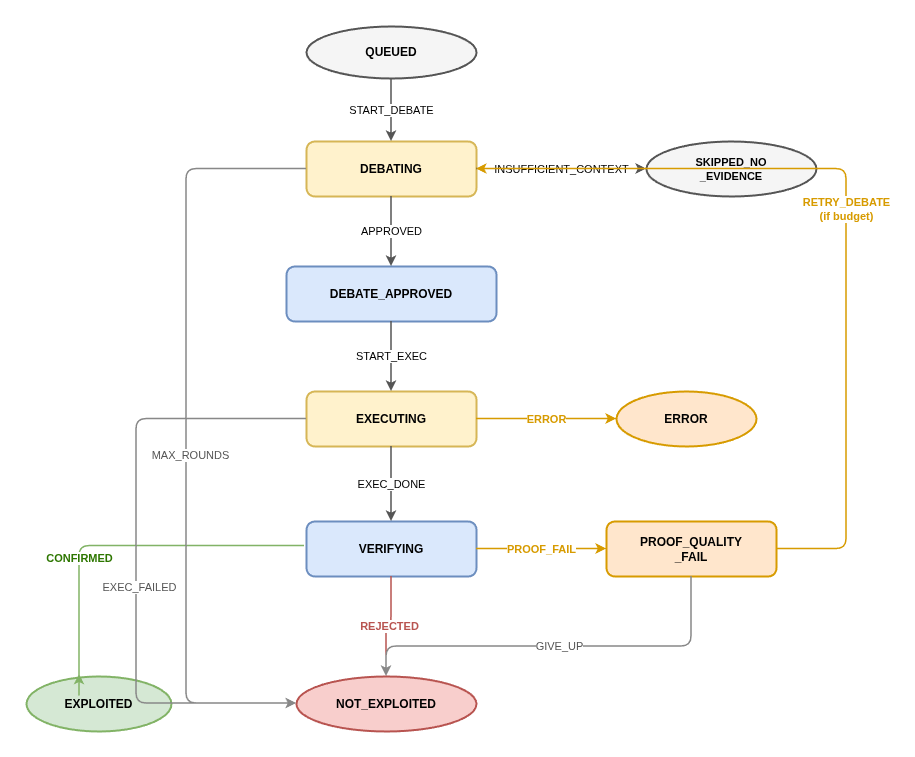
\includegraphics[width=0.85\linewidth]{src//images//chapter3/fig2_bug_graph.png}
    \caption{Vòng lặp khai thác per-bug với chu trình Debate -- Exec -- Verify}
    \label{fig:fig2_bug_graph}
\end{figure}

\textbf{Hình \ref{fig:fig2_bug_graph}} minh họa vòng lặp per-bug. Với mỗi BugDossier trong danh sách đã sắp xếp ưu tiên, hệ thống biên dịch và thực thi một sub-graph LangGraph riêng biệt gồm ba node chính: Debate, Exec, và Verify. Luồng chính là Debate nhận APPROVE → Exec → Verify ra kết quả. Khi Verify cho kết quả bằng chứng không đạt (ProofQualityFail), lý do từ chối của ProofGate được gửi ngược về Debate để Red agent điều chỉnh đúng điểm còn thiếu, tạo thành một chu trình phản hồi có kiểm soát. Toàn bộ routing trong sub-graph được thực hiện bởi các hàm Python tất định đọc giá trị enum từ trạng thái BugRun.

\subsection{Cơ chế tranh luận đối kháng (Debate)}

\begin{figure}[H]
    \centering
    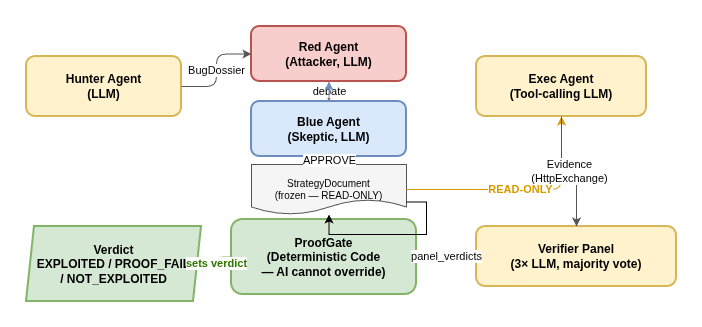
\includegraphics[width=1\linewidth]{src//images//chapter3/fig3_agents.png}
    \caption{Hai agent đối kháng trong giai đoạn Debate: Red (lập kế hoạch) và Blue (phản biện)}
    \label{fig:fig3_agents}
\end{figure}

Để đảm bảo tính khách quan và khả năng suy luận đa chiều, hệ thống không dựa vào một mô hình LLM đơn lẻ mà triển khai kiến trúc hai tác tử chuyên biệt với vai trò đối lập rõ ràng. Cơ chế phân tách này buộc mô hình ngôn ngữ phải thoát khỏi lối phân tích hời hợt và xem xét bài toán từ cả hai phía tấn công lẫn phòng thủ, từ đó sinh ra các kịch bản khai thác có tính khả thi cao hơn so với việc giao toàn bộ quyết định cho một agent duy nhất.

Giai đoạn Debate thực hiện một giao thức lập kế hoạch đối kháng giữa hai agent chuyên biệt, được minh họa trong \textbf{Hình \ref{fig:fig3_agents}}. Mục tiêu là đảm bảo chiến lược khai thác được kiểm tra kỹ lưỡng trước khi bất kỳ HTTP request thực nào được gửi đi, tránh lãng phí thời gian thực thi theo một kế hoạch có sai sót về cơ bản.

\textbf{Red agent} đóng vai trò người lập kế hoạch tấn công (nhiệt độ 0,6). Ở vòng đầu tiên, Red nhận BugDossier, thẻ pattern từ PlaybookProvider (bao gồm giải pháp tham khảo PortSwigger cho loại lỗ hổng đó), các cookie xác thực đã quan sát được trong quá trình reconnaissance, và bất kỳ kỹ thuật thành công nào từ bộ nhớ dài hạn. Red phải trả về một tài liệu chiến lược có cấu trúc bốn phần bắt buộc: \textit{STRATEGY} (tổng quan cách tiếp cận), \textit{EXECUTION GUIDE} (các bước cụ thể theo thứ tự), \textit{SUCCESS CONDITION} (điều kiện coi là khai thác thành công), và \textit{VERIFICATION QUESTIONS} (danh sách câu hỏi kiểm tra). Từ vòng thứ hai trở đi, Red chỉ phản hồi đúng các điểm Blue đã phản biện, không viết lại chiến lược từ đầu.

\textbf{Blue agent} đóng vai trò người phản biện (nhiệt độ 0,3). Blue nhận chiến lược của Red và cố tìm ra lý do chiến lược đó sẽ thất bại trong thực tế. Điểm mấu chốt là Blue và Red cùng nhìn vào đúng danh sách endpoint thực từ ReconArtifact, nên Blue có thể chỉ ra ngay khi Red đề xuất tấn công vào endpoint không tồn tại. Blue trả về một trong bốn phán quyết: \textit{APPROVE} (chiến lược đủ khả thi), \textit{REVISE} (có vấn đề cụ thể cần sửa), \textit{STOP} (không có cơ sở thực hiện), hoặc \textit{UNVERIFIABLE} (thiếu ngữ cảnh để đánh giá). Một ràng buộc bảo thủ được áp đặt cứng: nếu LLM trả về APPROVE ở vòng đầu tiên, phán quyết này bị ghi đè thành REVISE bất kể nội dung trả về là gì, đảm bảo luôn có ít nhất một vòng trao đổi đối kháng thực sự. Các phán quyết STOP và UNVERIFIABLE \textbf{không} bị ghi đè, vì chúng thể hiện quyết định rõ ràng cần được tôn trọng.

Ngoài ra, trước khi gửi phán quyết của Blue về DebateManager, một bước kiểm tra căn cứ trường (field-grounding check) tất định được thực hiện: tên các field tài chính mà Red đề cập trong chiến lược (được trích xuất bằng regex từ các đoạn text trong dấu backtick, JSON key trong ngoặc kép, hoặc phép gán giá trị số) được so sánh với danh sách field thực tế quan sát được trong form của ứng dụng từ ReconArtifact. Kiểm tra tập trung vào các field tài chính thường bị LLM ``bịa'' (ví dụ \texttt{unit\_price}, \texttt{subtotal}) do không quan sát được trong recon. Nếu có bất kỳ field nào Red đề cập không tồn tại trong form thực, phán quyết tự động bị ghi đè thành REVISE với một phản đối cụ thể về tên field, không phụ thuộc vào đánh giá của LLM.

Khi Blue phán quyết APPROVE, bốn phần của tài liệu chiến lược được đóng băng (frozen) vào BugRun như các trường bất biến: chiến lược tổng quan, hướng dẫn thực thi từng bước, điều kiện thành công, và danh sách câu hỏi xác minh. Exec agent sau đó nhận bốn trường này dưới dạng ngữ cảnh chỉ đọc và không thể thay đổi chúng trong quá trình thực thi.

\subsection{Thực thi khai thác (Execution)}

Giai đoạn Execution triển khai một vòng lặp tool-calling có giới hạn với nhiệt độ thấp để đảm bảo tính tái lập, trong đó Exec agent nhận chiến lược đã đóng băng, có trong tay bộ công cụ mở rộng (gửi HTTP request, điều khiển browser, đọc/ghi workspace, v.v.), và tự quyết định từng bước tiếp theo dựa trên response vừa nhận được.

\textbf{RecordingHttpClient} là thành phần trung tâm của giai đoạn này. Đây là một wrapper mỏng bao quanh \texttt{httpx.AsyncClient}, chặn mọi HTTP traffic từ Exec agent và ghi lại mỗi cặp request/response thành một \textit{HttpExchange} có số thứ tự tuần tự. Mỗi HttpExchange lưu đầy đủ: phương thức HTTP, URL, headers, body (qua BodyRef), status code, actor label (phiên đăng nhập nào gửi request này), danh sách 50 JSON key hàng đầu trong response, các field số (numeric fields) và các field định danh (ID fields) được trích xuất tự động, cùng với HTML title của response nếu có. Flag \texttt{follow\_redirects} được đặt về \texttt{False} có chủ đích: response 302 phải được ghi lại như một bằng chứng riêng, không được tự động theo dõi sang 200 tiếp theo, vì chính sự chuyển hướng đó là bằng chứng quan trọng cho một số loại lỗ hổng.

\textbf{Ngân sách bước và cửa sổ ngữ cảnh:} Exec agent được cấp tối đa 20 bước cho các pattern BLF chuỗi nhiều bước, và tối đa 12 bước cho các pattern BAC đơn giản hơn. Để tránh cạn kiệt token trong các chuỗi dài, một cửa sổ ngữ cảnh trượt giữ lại 8 lượt gần nhất cộng với system prompt và lượt user đầu tiên. \textbf{Guard chống bế tắc:} nếu đã thực hiện từ 7 bước trở lên mà chưa có bất kỳ request nào thay đổi trạng thái (POST/PUT/PATCH/DELETE trả về 2xx), vòng lặp kết thúc sớm để tránh lãng phí toàn bộ ngân sách vào việc chỉ gửi GET request không đem lại bằng chứng.

\textbf{Bốn loại ngữ cảnh bổ sung được inject vào prompt Exec:} (1) \textit{Endpoint schema} --- tên và kiểu của các field trong form, được thu thập từ nhiều nguồn: HTML form, JSON response, GET response schema, và form cross-page; (2) \textit{Known values} --- các giá trị cụ thể có thật từ ReconArtifact (ID tài nguyên, tên người dùng, giá trị enum hợp lệ, v.v.), được gán nhãn theo endpoint để tránh inject nhầm giá trị của endpoint này vào endpoint khác; (3) \textit{Chain steering} --- với các pattern BLF chuỗi nhiều bước (như tái sử dụng mã giảm giá, bỏ qua bước thanh toán), toàn bộ chuỗi bước trong \texttt{exploit\_approach} được inject kèm lệnh \textit{``không được dừng trước khi hoàn thành bước cuối cùng''}; (4) \textit{Memory skills} --- các kỹ thuật trừu tượng từ bộ nhớ dài hạn đã được xác nhận trên ít nhất hai target khác nhau.

\textbf{Tự động thương lượng encoding:} RecordingHttpClient xử lý một vấn đề kỹ thuật thực tế là Exec agent không biết endpoint nào dùng \texttt{application/x-www-form-urlencoded} và endpoint nào dùng \texttt{application/json}. Giải pháp: nếu một POST/PUT/PATCH trả về status code trong tập \{400, 404, 415, 422\}, request tự động được thử lại với encoding ngược lại. Exec agent chỉ thấy kết quả cuối cùng, không phải quá trình thử lại này.

\textbf{Fallback tất định:} Khi vòng lặp LLM kết thúc mà không tạo ra bằng chứng khai thác nào, hai routine tất định được gọi như phương án dự phòng. Routine \texttt{\_deterministic\_bac02\_attempt} (áp dụng cho pattern BAC-02) tìm cookie mang thông tin vai trò trong phiên xác thực, lật giá trị cookie (ví dụ chuyển \texttt{false} thành \texttt{true}, hoặc ghi đè giá trị role thành admin), sau đó gửi 2 request tuần tự: GET với cookie gốc (baseline) và GET với cookie đã lật (tamper) để đối chiếu response. Routine \texttt{\_deterministic\_blf\_attempt} thực hiện 3 request tuần tự: GET đọc trạng thái hiện tại (baseline), POST với payload chứa giá trị âm cho field tài chính hoặc số lượng, và GET đọc lại trạng thái mới (reread) để phát hiện state delta.

\subsection{Kiểm chứng bằng bằng chứng (Verification)}

\begin{figure}[H]
    \centering
    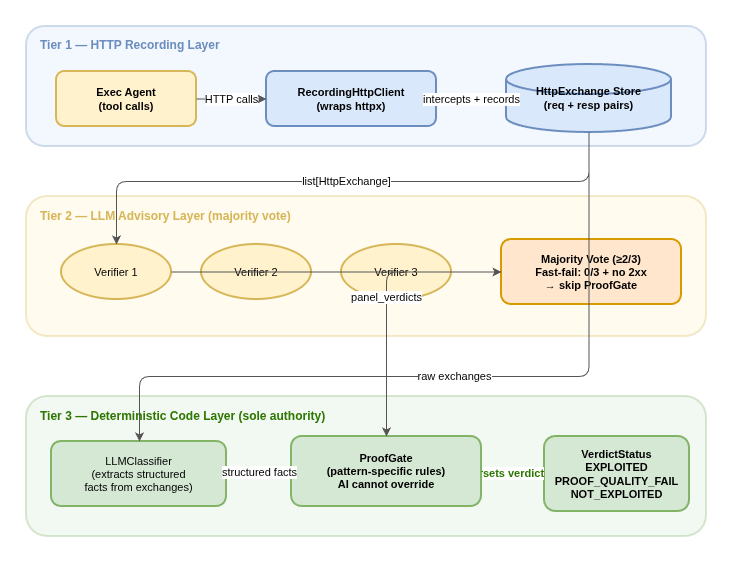
\includegraphics[width=1\linewidth]{src//images//chapter3/fig4_verification.png}
    \caption{Quy trình kiểm chứng hai bước: VerifierPanel tư vấn song song, sau đó ProofGate ra phán quyết tất định}
    \label{fig:fig4_verification}
\end{figure}

Giai đoạn Verification diễn ra theo hai bước tuần tự được thể hiện trong \textbf{Hình \ref{fig:fig4_verification}}.

\textbf{Bước 1 --- VerifierPanel song song:} Ba instance \textit{VerifierAgent} được dispatch đồng thời qua \texttt{asyncio.gather}, mỗi agent được gán một góc nhìn độc lập khác nhau: \textit{technical} (nhiệt độ 0,0 để có tính tái lập cao nhất), \textit{impact} (nhiệt độ 0,1), và \textit{skeptic} (nhiệt độ 0,2 để có sự đa dạng quan điểm). Quan trọng là mỗi Verifier không nhìn thấy transcript debate, tránh bị ảnh hưởng bởi lập luận của Red agent. Mỗi Verifier đọc tối đa 20 exchanges với response body đầy đủ tối đa 20.000 ký tự mỗi body, và trả về phán quyết gồm: xác nhận có/không, điểm tự tin (0--1), lập luận, danh sách ProofMarker được trích dẫn, các điểm phản bác, và câu trả lời cho từng câu hỏi xác minh trong \textit{VERIFICATION QUESTIONS} đã được đóng băng từ Debate. Kết quả tổng hợp theo quy tắc đa số: câu hỏi $i$ được coi là \textit{pass} khi tổng số Verifier trả lời ``có'' cho câu hỏi đó vượt quá $n/2$ (với $n=3$).

\textbf{Điều kiện fast-fail:} Nếu không có Verifier nào xác nhận VÀ không tồn tại bất kỳ exchange nào có status 2xx trong Evidence, hệ thống bỏ qua ProofGate và trả ngay kết quả ProofQualityFail, vì không có nền tảng HTTP nào để gate kiểm tra.

\textbf{Bước 2 --- ProofGate tất định và đường xác minh bổ sung:} Trừ trường hợp fast-fail, ProofGate luôn được chạy kể cả khi cả ba Verifier đều từ chối, vì gate hoạt động trên dữ liệu thô và có thể tìm ra bằng chứng mà LLM bỏ sót. Phán quyết cuối cùng được tổng hợp theo quy tắc ưu tiên: (1) nếu ProofGate báo EXPLOITED thì kết quả là EXPLOITED; (2) nếu ProofGate không báo EXPLOITED nhưng panel LLM đạt đủ ngưỡng xác minh ($\geq 2$ câu hỏi trong VERIFICATION QUESTIONS được xác nhận bởi đa số Verifier) thì kết quả vẫn là EXPLOITED qua đường xác minh câu hỏi --- cơ chế này cho phép phán quyết dựa trên cấu trúc đối kháng đã được kiểm chứng khi panel nhìn thấy bằng chứng ngữ cảnh mà gate không kiểm tra được (ví dụ: nội dung response phi tiếng Anh); (3) nếu ProofGate báo InfoExposureOnly thì kết quả là InfoExposureOnly; (4) còn lại là ProofQualityFail để kích hoạt retry.

%----------------------------------------------------------------------------------------
\section{Cổng chứng minh (ProofGate)}
%----------------------------------------------------------------------------------------

Nhằm khắc phục hạn chế cốt lõi của các mô hình học sâu --- xu hướng bịa đặt thông tin (hallucination) và thiếu ổn định khi đưa ra kết luận bảo mật --- hệ thống đề xuất và triển khai một cơ chế xác minh hai tầng kết hợp điều phối trạng thái chặt chẽ: tầng tư vấn đa Verifier LLM chạy song song để đánh giá ngữ nghĩa, và tầng ProofGate tất định bằng mã nguồn để ra phán quyết cuối cùng dựa trên bằng chứng HTTP quan sát được. Không một quyết định nào của AI được chấp nhận nếu không có sự đối chiếu tất định.

ProofGate là thành phần đảm bảo hệ thống không bao giờ báo cáo một lỗ hổng mà không có bằng chứng HTTP cụ thể. Mỗi pattern lỗ hổng có một subclass ProofGate riêng với các điều kiện kiểm tra được định nghĩa trong code, không phải trong prompt LLM.

\renewcommand{\arraystretch}{1.5}
\begin{longtable}{
  >{\raggedright\arraybackslash}p{2.8cm}
  >{\raggedright\arraybackslash}p{3.2cm}
  >{\raggedright\arraybackslash}p{8.8cm}
}
\caption{Toàn bộ các pattern lỗ hổng được hỗ trợ trong ProofGate (20 pattern)}
\label{tab:proof_rules} \\

\toprule
\textbf{Pattern} & \textbf{ProofKey bắt buộc} & \textbf{Điều kiện chấp nhận} \\
\midrule
\endfirsthead

\multicolumn{3}{l}{\textit{(tiếp theo Bảng \ref{tab:proof_rules})}} \\
\toprule
\textbf{Pattern} & \textbf{ProofKey bắt buộc} & \textbf{Điều kiện chấp nhận} \\
\midrule
\endhead

\midrule
\multicolumn{3}{r}{\textit{(còn tiếp)}} \\
\endfoot

\bottomrule
\endlastfoot

% --- BAC ---
\multicolumn{3}{l}{\textbf{Nhóm BAC (Broken Access Control) --- BACProofGate}} \\
\midrule

BAC-01, BAC-06, BAC-07 &
  PrivilegedAccess &
  Actor không có quyền nhận HTTP 200 trên trang admin/nhạy cảm; body chứa $\geq 2$ bản ghi có field nhạy cảm (email, balance, role, ...) hoặc title trang xác nhận nội dung quản trị. Nếu eval này thất bại, tự động thử IDOR --- nếu tìm thấy cross-user evidence thì tái phân loại sang BAC-03. \\[4pt]

BAC-02 &
  PrivilegedAccess, AuthBypass &
  Trang đặc quyền được render cho actor thường sau khi tamper cookie mang thông tin vai trò. Phát hiện theo thứ tự bất kỳ: tìm cặp exchange cùng endpoint, Cookie khác nhau, một trả 403/302 và một trả 200 với nội dung đặc quyền. \\[4pt]

BAC-03 &
  OwnershipBypass &
  Response chứa field chủ sở hữu (userId, ownerId, createdBy, ...) có giá trị khác với user ID attacker; hoặc $\geq 2$ exchange trên cùng endpoint template trả về identity khác nhau (email, username). Phát hiện qua 4 lớp: JSON owner-field mismatch, HTML identity-change fallback, redirect-body fallback, và LLM Classifier fallback. \\[4pt]

BAC-05 &
  OwnershipBypass, SensitiveFieldExposed &
  IDOR kết hợp lộ thông tin nhạy cảm trên endpoint đa bước: cùng yêu cầu cả cross-user access lẫn exposed PII fields (password, token, secret key). \\[4pt]

BAC-08 &
  OwnershipBypass, SensitiveFieldExposed &
  IDOR kết hợp lộ thông tin xác thực (password, token, secret key) của victim trong response. \\[4pt]

BAC-04 &
  AuthBypass &
  Request chứa header \texttt{X-HTTP-Method-Override} hoặc tham số \texttt{?\_method=} được server chấp nhận; hoặc cùng endpoint với method khác nhau trả về status code khác nhau (403 vs 200). Chỉ yêu cầu AuthBypass (không yêu cầu thêm PrivilegedAccess), vì bản thân việc method bypass thành công chứng minh lỗ hổng. \\[4pt]

\midrule
% --- BLF ---
\multicolumn{3}{l}{\textbf{Nhóm BLF (Business Logic Flaw) --- BLFProofGate}} \\
\midrule

BLF-01 &
  PriceManipulation, StateDelta &
  Giá trị âm hoặc bằng 0 trong field tài chính (amount, price, total) được server trả 2xx/3xx, không có error marker trong response body. Hệ thống kiểm tra cả field tiền tệ lẫn field số lượng để xử lý trường hợp Hunter phân loại nhầm BLF-01/BLF-06. \\[4pt]

BLF-02 &
  QuantityTamper, StateDelta &
  Server chấp nhận giá trị không hợp lệ về kiểu hoặc nằm ngoài dải cho phép: giá trị đặc biệt (\texttt{null}, \texttt{none}, \texttt{undefined}, \texttt{NaN}, \texttt{Infinity}) hoặc giá trị decimal trong field integer ($f \neq i$ với $0 < |f| < 10^6$) được trả 2xx không có error marker. \\[4pt]

BLF-03, BLF-09 &
  StateSkip, StateDelta &
  $\geq 2$ endpoint action khác nhau (POST/PUT/PATCH/DELETE) trả về 2xx kết hợp với state delta không rỗng, chứng minh một bước bắt buộc trong workflow đã bị bỏ qua. \\[4pt]

BLF-04 &
  StateDelta &
  Cùng endpoint nhận $\geq 2$ request thay đổi trạng thái (POST/PUT/PATCH) trả về 2xx thành công, cho thấy không có cơ chế chống tiêu thụ nhiều lần (guard one-time-use absent) hoặc state delta ghi nhận phần tài nguyên thay đổi bất thường. \\[4pt]

BLF-05 &
  PriceManipulation, StateDelta &
  Cùng mã coupon được server trả 2xx $\geq 2$ lần với ít nhất một sự kiện consume (checkout/purchase/confirm/pay/order) xuất hiện giữa hai lần áp dụng; hoặc $\geq 2$ mã khác nhau được stack đồng thời; hoặc tổng đơn hàng $\leq 0$. \\[4pt]

BLF-06, BLF-07, BLF-08 &
  QuantityTamper, StateDelta &
  Số lượng âm hoặc giá trị gây tràn số (integer overflow) được server chấp nhận (2xx/3xx không có error marker). BLF-08 đặc biệt kiểm tra hiện tượng wrap-around số học dẫn đến tổng giỏ hàng âm. \\[4pt]

BLF-10, BLF-11, BLF-12 &
  PrivilegedAccess, AuthBypass &
  Leo thang đặc quyền thông qua lỗ hổng logic nghiệp vụ: bỏ qua tham số phân quyền (BLF-10), đăng ký tài khoản với email bị cắt ngắn để vượt qua kiểm tra domain (BLF-11), hoặc bỏ qua request chọn role trong luồng đăng nhập nhiều bước (BLF-12). \\

\end{longtable}
\renewcommand{\arraystretch}{1}

\textbf{Bảng \ref{tab:proof_rules}} tóm tắt các điều kiện cho từng pattern. Nguyên tắc chung: tất cả ProofKey bắt buộc phải được thỏa mãn đồng thời để có kết quả EXPLOITED; nếu chỉ thỏa một phần, kết quả là InfoExposureOnly; không thỏa điều kiện nào là Failed.

\subsection{Phân loại thực thể bằng LLM (Classifier)}

Đối với các pattern phức tạp hơn như BAC-03 (IDOR), ProofGate có một cơ chế fallback: gọi \textit{ClassifyResponses} khi việc so sánh field trực tiếp không đủ kết luận. Classifier chọn tối đa 3 exchange có status 2xx (sắp xếp theo độ dài response body giảm dần, không trùng cặp URL--actor), giới hạn 6.000 ký tự mỗi body, và cung cấp một JSON schema mô tả các fact cần trích xuất theo từng pattern (ví dụ BAC-03 cần \texttt{owner\_field\_name}, \texttt{owner\_field\_value}, \texttt{email\_in\_response}). Nhiệt độ được đặt là 0,0 cho lần thử đầu, tăng lên 0,4 cho các lần thử lại (tối đa 3 lần gọi LLM). Điểm quan trọng là các fact trích xuất vẫn được đưa vào kiểm tra bởi đúng các luật tất định của gate --- Classifier chỉ là bộ trích xuất đặc trưng (feature extractor), không phải bộ phán quyết.

%----------------------------------------------------------------------------------------
\section{Hệ thống bộ nhớ dài hạn (Long-term Memory)}
%----------------------------------------------------------------------------------------

Sau mỗi lần chạy hoàn chỉnh, hệ thống tích lũy kinh nghiệm vào một cơ sở dữ liệu SQLite để cải thiện hiệu suất cho các target tiếp theo. Kiến trúc bộ nhớ gồm hai tầng với cơ chế phân cấp nhằm tránh hiện tượng overfitting vào một ứng dụng cụ thể.

\subsection{Tầng 1 --- Bộ nhớ episodic (theo target)}

Mỗi lần khai thác được ghi lại thành một \textit{Episode} trong bảng \texttt{episodes}, được xác định bởi \textit{target fingerprint} --- một hash dựa trên host, title trang, và danh sách endpoint đã sắp xếp của target đó. Mỗi Episode lưu: mã pattern, họ endpoint (family path), payload đã dùng, tập ProofMarker đã thỏa, và kết quả. Một cổng ghi quan trọng được áp đặt tại caller: \textbf{chỉ các Episode có kết quả EXPLOITED hoặc InfoExposureOnly từ ProofGate mới được ghi vào store}. Nếu chỉ có panel LLM xác nhận mà ProofGate không chấp thuận, Episode không được ghi, ngăn chặn kiến thức không được kiểm chứng lan vào bộ nhớ. Tầng truy xuất cũng bổ sung lọc: khi inject vào Hunter chỉ lấy Episode có outcome \textit{exploited} hoặc \textit{info}; khi inject vào Exec chỉ lấy outcome \textit{exploited}.

Khi chạy lại trên cùng target, hệ thống lấy các Episode thành công trước đó và inject payload và endpoint cụ thể vào prompt Exec dưới dạng ngữ cảnh ưu tiên cao.

\subsection{Tầng 2 --- Bộ nhớ semantic (xuyên target)}

Để hệ thống học được kỹ thuật tổng quát thay vì chỉ nhớ các giá trị cứng của một ứng dụng, tầng 2 thực hiện promotion (thăng cấp) các Episode thành các \textit{Rule} trừu tượng theo điều kiện:

\textbf{Điều kiện thăng cấp:} (i) pattern-endpoint family đó đã được xác nhận thành công ít nhất 3 lần; VÀ (ii) trong số các lần thành công đó, có ít nhất 2 target fingerprint khác nhau (tức là thành công trên ít nhất 2 ứng dụng riêng biệt). Điều kiện này ngăn chặn trường hợp một kỹ thuật chỉ hoạt động trên một ứng dụng duy nhất vô tình được coi là kỹ thuật phổ quát.

Trước khi lưu, thông tin target-specific được strip bỏ: host, URL đầy đủ, title ứng dụng đều bị xóa. Hàm \texttt{\_endpoint\_role()} chuẩn hóa đường dẫn bằng cách loại bỏ các segment noise (\texttt{api}, \texttt{v1}, \texttt{v2}, \texttt{\{id\}}, \texttt{\{uuid\}}) và lấy segment cuối cùng làm vai trò endpoint --- ví dụ hai endpoint chuyển tiền trên hai ứng dụng khác nhau đều được chuẩn hóa về role \texttt{transfer}. Mẫu kỹ thuật trừu tượng (\texttt{\_abstract\_technique()}) khác nhau theo pattern: BLF-01/05 sinh câu mô tả theo loại giá trị (âm, zero, extreme), BAC-02 mô tả ``gửi cookie đã tamper'', BAC-03 mô tả ``thay đổi path id sang user khác''. Kết quả là các Rule như \textit{``giá trị âm trên field tài chính của endpoint transfer''} thay vì \textit{``gửi amount=-100 tới một host cụ thể''. Các Rule đã thăng cấp được inject vào prompt Exec của các lần chạy tiếp theo trên target mới dưới phần \textit{Past Successful Techniques}. Hệ thống cũng tự động dọn dẹp bộ nhớ theo thời gian: Episode cũ hơn 90 ngày và attempt thất bại cũ hơn 14 ngày bị xóa, đảm bảo cơ sở kinh nghiệm không bị lỗi thời.
